% !TeX root = ../main.tex
% !TeX program = pdflatex
% !TeX encoding = UTF-8
% Biên dịch tài liệu gốc bằng pdfLaTeX.

\chapter{Hướng dẫn cài đặt và sử dụng chương trình}
\label{chap:program-instructions}

\section{Yêu cầu môi trường}

Chương trình gồm một frontend React và một backend Python chạy thành hai tiến
trình riêng. Máy thử nghiệm cần có trình duyệt hiện đại, kết nối được đến hai
cổng cục bộ và các công cụ trong Bảng~\ref{tab:environment-requirements}.
Project không sử dụng database nên không có bước cài đặt hoặc khởi tạo cơ sở
dữ liệu.

\begin{table}[h!]
\centering
\caption{Môi trường và thư viện cần thiết}
\label{tab:environment-requirements}
\begin{tabular}{>{\raggedright\arraybackslash}p{4.1cm}
                >{\raggedright\arraybackslash}p{4.0cm}
                >{\raggedright\arraybackslash}p{6.0cm}}
\toprule
Thành phần & Phiên bản & Vai trò \\
\midrule
Python & 3.10 trở lên & Chạy HTTP API và các thuật toán tìm kiếm. \\
Node.js, npm & Node.js 18 trở lên & Cài package, chạy Vite và build frontend. \\
React & 19.x & Xây dựng giao diện theo component. \\
Vite & 6.x & Development server, proxy API và production build. \\
Zustand & 5.x & Quản lý state chung của giao diện và mô phỏng. \\
NetworkX & Từ 3.2 đến dưới 4 & Biểu diễn đồ thị có hướng trong backend. \\
pandas & Từ 2.0 đến dưới 3 & Đọc và kết hợp các bảng dữ liệu CSV. \\
\bottomrule
\end{tabular}
\end{table}

Các phiên bản frontend được khai báo trong \texttt{package.json}; hai thư viện
Python được khóa khoảng phiên bản trong \texttt{requirements.txt}. Backend sử
dụng \texttt{ThreadingHTTPServer} của thư viện chuẩn Python, không sử dụng
FastAPI hoặc Flask.

\section{Tải mã nguồn và cài đặt dependencies}

Mở Windows PowerShell tại thư mục muốn lưu project và thực hiện:

\begin{verbatim}
git clone https://github.com/YongQi241/AIPRO-Route_DaLat.git
cd AIPRO-Route_DaLat
\end{verbatim}

Tại thư mục gốc của repository, tạo virtual environment và cài dependencies
backend:

\begin{verbatim}
python -m venv .venv
.\.venv\Scripts\Activate.ps1
python -m pip install -r requirements.txt
\end{verbatim}

Tiếp theo cài dependencies frontend:

\begin{verbatim}
npm.cmd install
\end{verbatim}

Tất cả đường dẫn dữ liệu backend được tính tương đối từ vị trí project. Người
dùng không cần sao chép CSV hoặc GeoJSON sang một thư mục khác.

\section{Khởi động backend}

Mở terminal PowerShell thứ nhất tại thư mục gốc của project:

\begin{verbatim}
.\.venv\Scripts\Activate.ps1
python -m backend.server
\end{verbatim}

Mặc định backend lắng nghe tại \texttt{http://127.0.0.1:8000}. Khi khởi động
thành công, terminal in dòng \texttt{Route API listening on
http://127.0.0.1:8000}. Có thể kiểm tra trạng thái bằng:

\begin{verbatim}
Invoke-RestMethod http://127.0.0.1:8000/api/health
\end{verbatim}

Response hợp lệ có \texttt{status} bằng \texttt{ok}, tên dịch vụ
\texttt{dalat-route-api} và phiên bản API \texttt{2.0}. Backend cung cấp ba
endpoint chính:

\begin{itemize}[itemsep=2pt]
  \item \texttt{GET /api/health}: kiểm tra tình trạng dịch vụ;
  \item \texttt{GET /api/algorithms}: xem thuật toán và khả năng được backend
  hỗ trợ;
  \item \texttt{POST /api/routes/solve}: nhận yêu cầu và trả kết quả tìm đường.
\end{itemize}

\section{Khởi động frontend}

Giữ backend đang chạy và mở terminal PowerShell thứ hai tại thư mục gốc:

\begin{verbatim}
npm.cmd run dev
\end{verbatim}

Vite hiển thị địa chỉ truy cập trong terminal; với cấu hình mặc định, mở
\texttt{http://localhost:5173}. Trong development, Vite tự chuyển tiếp
\texttt{/api/*} đến backend ở cổng 8000. Để dừng một server, chọn terminal của
nó và nhấn \texttt{Ctrl+C}.

Các lệnh kiểm tra frontend được khai báo sẵn:

\begin{verbatim}
npm.cmd test
npm.cmd run build
\end{verbatim}

Lệnh thứ nhất chạy test timeline, Zustand và cơ chế mở tab kết quả. Lệnh thứ
hai tạo bản production trong thư mục \texttt{dist/}. Nếu frontend và backend
được triển khai khác origin, có thể cấu hình biến
\texttt{VITE\_ROUTE\_API\_URL} trước khi chạy/build frontend.

\section{Các file dữ liệu được sử dụng}

\begin{table}[h!]
\centering
\caption{Vai trò của các file dữ liệu trong hệ thống}
\label{tab:runtime-data-files}
\begin{tabular}{>{\raggedright\arraybackslash}p{5.5cm}
                >{\raggedright\arraybackslash}p{9.0cm}}
\toprule
File & Vai trò \\
\midrule
\path{nodes_snapped.geojson} &
Chứa 25 địa điểm, ID, tên và tọa độ để frontend tạo danh sách chọn và vẽ node. \\
\path{edges.geojson} &
Chứa hình học của 114 cạnh có hướng. Frontend dùng \texttt{edge\_id} để vẽ
mạng đường và chọn chính xác cạnh thuộc tuyến. \\
\path{nodes_snapped.csv}, \path{edges.csv} &
Nguồn dữ liệu node và cạnh mà backend dùng để xây dựng
\texttt{NetworkX DiGraph}. \\
\path{edge_conditions.csv} &
Chứa điều kiện từng cạnh theo năm kịch bản S0--S4; backend dùng để điều chỉnh
thời gian, risk, chi phí và loại cạnh bị đóng. \\
\path{data/mock-result.json} &
Fixture cố định cho kiểm thử frontend. Chỉ được dùng làm fallback development
khi API không thể kết nối và yêu cầu là DL01--DL09 không có điểm trung gian. \\
\bottomrule
\end{tabular}
\end{table}

Hai file GeoJSON frontend đọc nằm trong
\texttt{data/generated/} và được tải tự động khi ứng dụng
mở. Vì vậy giao diện hiện không cần nút Load data. Năm kịch bản là S0
(ngày thường bình thường), S1 (cuối tuần đông), S2 (giờ cao điểm buổi tối), S3
(mưa lớn) và S4 (sương mù dày).

\section{Hướng dẫn sử dụng giao diện}

\begin{enumerate}[itemsep=3pt]
  \item Khởi động backend và frontend theo hai phần trên, sau đó mở địa chỉ Vite.
  Chờ thông báo nạp dữ liệu kết thúc và kiểm tra mạng đường Đà Lạt đã xuất hiện.
  \item Chọn Start location và Destination bằng hai danh sách thả xuống. Hai
  điểm phải khác nhau. Giao diện hiện không chọn đầu mút bằng cách bấm trực tiếp
  lên node trên bản đồ.
  \item Nếu cần đi qua nhiều địa điểm, chọn từng Intermediate location rồi bấm
  Add. Chỉ Nearest Neighbor và Brute Force TSP sử dụng danh sách này; với hai
  thuật toán đó, frontend tự thêm Destination vào tập đích cần thăm. Brute Force
  TSP nhận tối đa tám đích.
  \item Chọn một trong năm Scenario và một Optimization. Các lựa chọn tiêu chí
  gồm Balanced, Shortest distance, Fastest time và Lowest cost; \texttt{cost}
  là alias của profile \texttt{balanced} trong backend.
  \item Chọn thuật toán trong Search strategy. Giao diện hiện có BFS, DFS, UCS,
  Dijkstra, A*, Nearest Neighbor, Hill Climbing và Brute Force TSP. Backend còn
  hỗ trợ Greedy Best-First qua API nhưng sidebar chưa có lựa chọn này.
  \item Nhấn Find route. Frontend gửi ID thay vì tên địa điểm đến API. Trong lúc
  chờ, form bị vô hiệu hóa; khi nhận response, Status message cho biết thành
  công, không có đường, input không hợp lệ hoặc lỗi dịch vụ.
  \item Với kết quả có trace, giao diện tự Play. Có thể Pause để quan sát thủ
  công, sau đó dùng First action, Previous action, Next action hoặc Last action.
  Chọn Speed để đổi tốc độ giữa $0.5\times$, $1\times$, $1.5\times$ và
  $2\times$; Reset đưa mô phỏng về đầu.
  \item Theo dõi màu node Unvisited, Frontier, Visited, Current và Final-route
  node. Candidate edge là các cạnh có thể xét từ node hiện tại; Active
  relaxation là cạnh đang được xét. Tuyến cuối chỉ dùng các ID trong
  \texttt{path\_edges}; đoạn cảnh báo được tô cam khi congestion từ 4 trở lên
  hoặc risk lớn hơn 0.
  \item Hai tab Simulation và Algorithm trace trình bày tác vụ hiện tại, tiến
  độ, frontier, visited và log action. Sau khi timeline lần đầu tới cuối, ba tab
  Output, Breakdown và Human-readable reasoning được mở để xem tuyến, tổng chỉ
  số, dữ liệu từng đoạn và giải thích từ backend.
  \item Chọn Map để xem tọa độ địa lý hoặc Graph để xem topology được giãn đều.
  Dùng nút $+$/$-$ hoặc con lăn để zoom; giữ chuột trái và kéo để di chuyển;
  dùng Reset view hoặc nhấn đúp để trở về góc nhìn ban đầu.
  \item Khi cần thêm diện tích cho bản đồ, dùng nút tam giác để thu gọn Route
  controls phía trên, Search strategy bên phải hoặc Search details phía dưới.
\end{enumerate}

Nếu backend không chạy trong development, frontend có thể hiển thị fixture cho
DL01--DL09. Với mọi yêu cầu khác, chế độ demo trả \texttt{invalid\_input} thay
vì tự tính tuyến. Production build không che giấu lỗi kết nối API bằng fixture.

\section{Ví dụ tìm đường một điểm đích}

Bảng~\ref{tab:single-route-example} lấy từ một lần gọi trực tiếp
\texttt{calculate\_route} của backend với dữ liệu hiện tại. Đây không phải
fixture frontend. Thời gian xử lý phụ thuộc phần cứng và có thể thay đổi giữa
các lần chạy; những thông số tuyến còn lại được tính từ dataset và request đã
nêu.

\begin{table}[h!]
\centering
\caption{Ví dụ kết quả A* một điểm đích từ backend}
\label{tab:single-route-example}
\begin{tabular}{>{\raggedright\arraybackslash}p{4.0cm}
                >{\raggedright\arraybackslash}p{10.3cm}}
\toprule
Trường & Giá trị \\
\midrule
Điểm bắt đầu & Nhà lao thiếu nhi Đà Lạt (DL01) \\
Điểm đích & Làng Cu Lần (DL09) \\
Thuật toán & A* \\
Kịch bản, tiêu chí & S0, \texttt{balanced} \\
Tuyến node & DL01 $\rightarrow$ DL06 $\rightarrow$ DL19 $\rightarrow$ DL09 \\
Tên địa điểm & Nhà lao thiếu nhi Đà Lạt $\rightarrow$ Thung Lũng Tình Yêu
$\rightarrow$ Làng Đồng trụ LangBiang $\rightarrow$ Làng Cu Lần \\
Cạnh tuyến & E005, E041, E064 \\
Tổng khoảng cách & 39.429 km \\
Thời gian ước tính & 68.307 phút \\
Tổng chi phí & 1.34248 \\
Tổng risk & 1.0 \\
Số node đã xét & 25 \\
Thời gian xử lý đo được & 0.637 ms \\
\bottomrule
\end{tabular}
\end{table}

Với tiêu chí \texttt{balanced}, A* dùng \texttt{route\_cost}. Source hiện dùng
zero heuristic cho trọng số \texttt{route\_cost}/risk để bảo toàn điều kiện
không đánh giá vượt chi phí còn lại. Backend cũng trả phần giải thích so sánh
tuyến được chọn với tuyến ngắn nhất theo khoảng cách; frontend chỉ định dạng và
hiển thị nội dung này.

\section{Ví dụ nhiều địa điểm}

Chức năng nhiều địa điểm đã được triển khai ở cả frontend và backend. Ví dụ
trong Bảng~\ref{tab:multi-route-example} dùng Nearest Neighbor, bắt đầu tại
DL01, chọn DL03 và DL08 làm điểm trung gian, DL09 làm điểm đích; frontend gửi
tập \texttt{visit\_nodes} là DL03, DL08 và DL09.

\begin{table}[h!]
\centering
\caption{Ví dụ kết quả nhiều địa điểm từ backend}
\label{tab:multi-route-example}
\begin{tabular}{>{\raggedright\arraybackslash}p{4.0cm}
                >{\raggedright\arraybackslash}p{10.3cm}}
\toprule
Trường & Giá trị \\
\midrule
Điểm bắt đầu & Nhà lao thiếu nhi Đà Lạt (DL01) \\
Tập địa điểm cần thăm & DL03, DL08, DL09 \\
Thuật toán & Nearest Neighbor \\
Kịch bản, tiêu chí & S1, \texttt{time} \\
Thứ tự ghé thăm & DL01 $\rightarrow$ DL03 $\rightarrow$ DL08
$\rightarrow$ DL09 \\
Tuyến node đầy đủ & DL01 $\rightarrow$ DL02 $\rightarrow$ DL22
$\rightarrow$ DL21 $\rightarrow$ DL03 $\rightarrow$ DL04
$\rightarrow$ DL18 $\rightarrow$ DL08 $\rightarrow$ DL20
$\rightarrow$ DL09 \\
Tổng khoảng cách & 43.778 km \\
Thời gian ước tính & 91.424 phút \\
Tổng chi phí & 2.057684 \\
Tổng risk & 9.0 \\
Số cạnh tuyến & 9 \\
Thời gian xử lý đo được & 4.108 ms \\
\bottomrule
\end{tabular}
\end{table}

Nearest Neighbor lần lượt chọn đích chưa thăm có chi phí đường đi Dijkstra nhỏ
nhất từ vị trí hiện tại, nên đây là phương pháp xấp xỉ và không đảm bảo tối ưu
toàn cục. Để xác minh chế độ chính xác, cùng request trên đã được chạy với Brute
Force TSP: backend xét đủ 6 hoán vị, trả cùng thứ tự và cùng tổng thời gian
91.424 phút trong lần thử này, với thời gian xử lý 4.965 ms. Kết quả Brute Force
TSP là tối ưu toàn cục cho tập đích và trọng số đã chọn, trong giới hạn tối đa
tám đích của chương trình.

\section{Ảnh chụp hệ thống}

Ba file ảnh hiện có trong \path{report/images/} vẫn là ảnh placeholder
có chữ mô tả, không phải ảnh chụp chương trình đang chạy. Trước khi nộp, nhóm
cần chạy hệ thống và thay chúng bằng ảnh chụp tương ứng:

\begin{itemize}[itemsep=2pt]
  \item \texttt{screenshot\_main\_window.png}: giao diện chính sau khi đồ thị
  được tải;
  \item \texttt{screenshot\_route\_result.png}: tuyến cuối cùng, chỉ số và tab
  kết quả sau khi mô phỏng hoàn tất;
  \item \texttt{screenshot\_multi\_location.png}: một request Nearest Neighbor
  hoặc Brute Force TSP có điểm trung gian.
\end{itemize}

% TODO trước khi nộp: thay ba ảnh placeholder bằng ảnh chụp thật rồi bỏ dấu
% comment ở các lệnh includegraphics tương ứng.
% 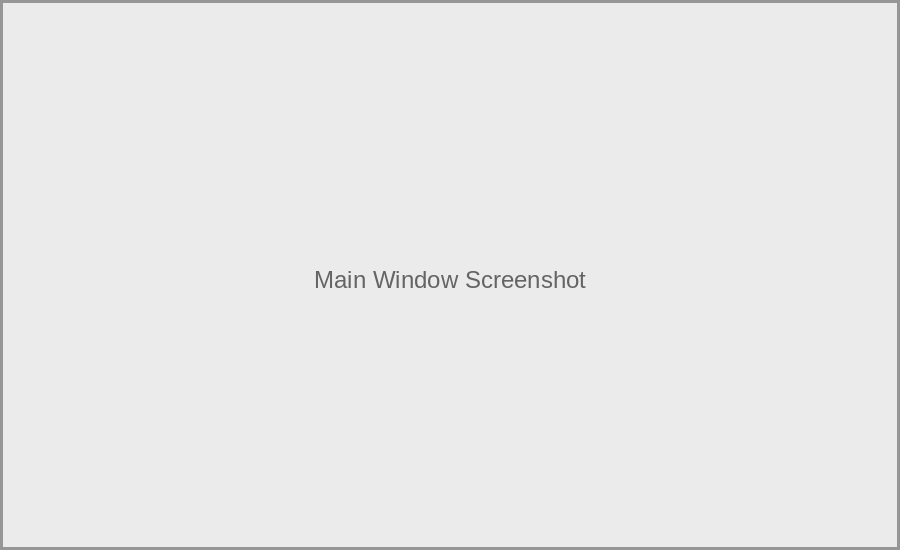
\includegraphics[width=0.85\textwidth]{images/screenshot_main_window.png}
% 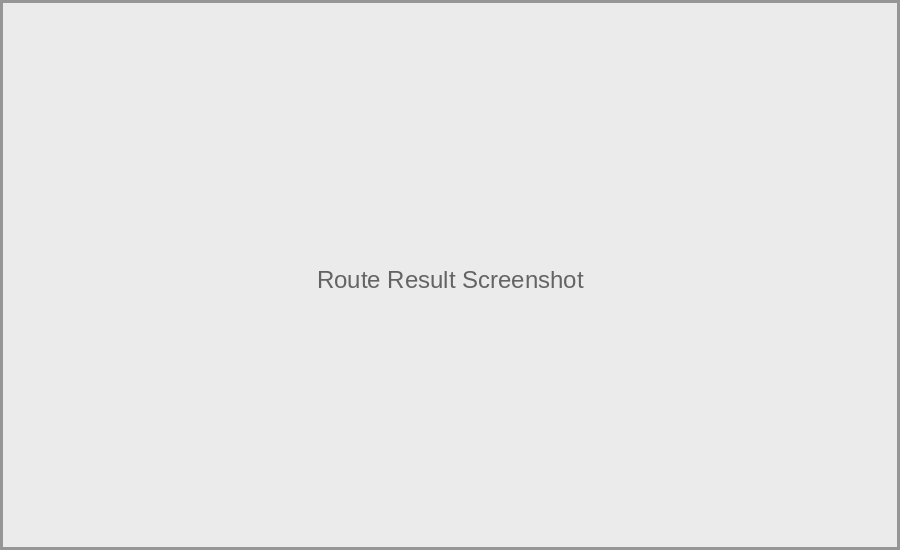
\includegraphics[width=0.85\textwidth]{images/screenshot_route_result.png}
% 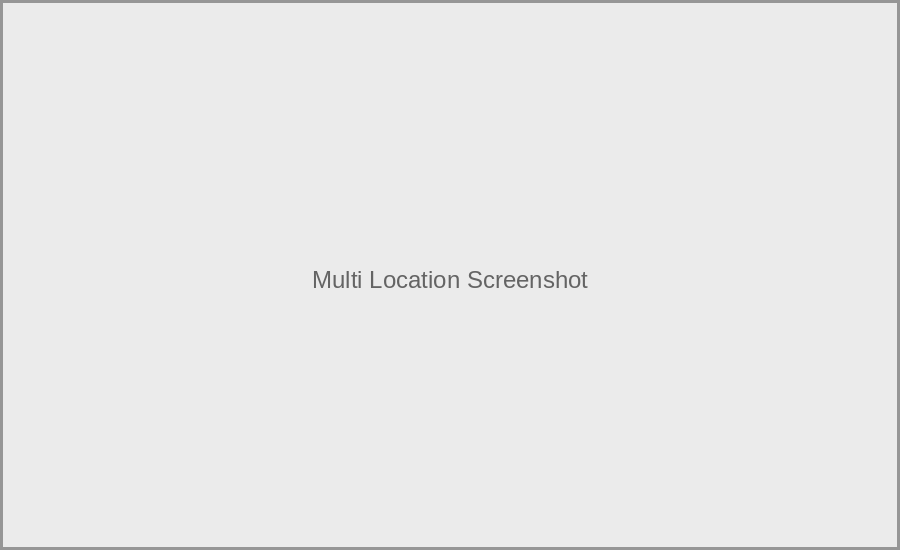
\includegraphics[width=0.85\textwidth]{images/screenshot_multi_location.png}
